%%%%
% Преамбула: подключение необходимых пакетов
% Редактируйте осторожно!
%

\documentclass[hyperref={unicode}]{beamer}

\usepackage[utf8x]{inputenc}
\usepackage[english, russian]{babel}
\usepackage{color, colortbl}
\usepackage{rotating} 
\usepackage{graphicx}
\usepackage{algorithmic}

\usetheme[nosecheader]{PetrSU-CS}


%%%%
% Преамбула: основные параметры презентации
% Отредактируйте в соответствии с комментариями
%

\title[%
    % Краткое название работы не используется в этой презентации!
    Бобры и Интернет
]{%
    % Полное название работы отображается на титульной странице
	Персонализированный трекер\\
	пользователя
}

% Подзаголовком опишите тип работы:
% - Курсовая работа
% - Выпускная квалификационная работа бакалавра
% - Дипломная работа
% - Магистерская диссертация
\subtitle{Промежуточный отчет о научно-исследовательской работе}

\author[%
    % Имя и фамилия автора работы отображаются на каждом слайде в нижнем колонтитуле
    Владислав Клименко
]{%
    % Имя, отчество и фамилия автора работы отображаются на титульном слайде
    Владислав Викторович Клименко
}

\date[%
    % Дата защиты
    01.06.2018
]{%
    % Руководитель
    Научный руководитель: д.ф.-м.н., преподаватель  В. М. Димитров
}

\institute[%
    % Краткое название организации не используется в этой презентации
    ПетрГУ
]{%
    % Полное название организации и подразделения
    Петрозаводский государственный университет\\
    Кафедра информатики и математического обеспечения
}


%%%%
%
% Начало содержимого слайдов
%

\begin{document}

% Титульный слайд
\begin{frame}
\maketitle
\end{frame}

% Пример слайда для обоснования актуальности работы
\begin{frame}
  % Заголовок слайда
  \frametitle{Понятие трекера}
  Трекер - это программа позволяющая отслеживать путь пользователя и выводить
  различную информацию о том, каким образом он перемещался.
\end{frame}

% Пример слайда с формулировкой целей и задач
\begin{frame}
  % Заголовок слайда
  \frametitle{Цель и задачи}
  \framesubtitle{(формулируем цель работы и задачи для достижения цели)}
  \begin{block}{Цель работы}
    Разработать энергоэффективный трекер, который может
    постоянно опрашивать координаты пользователя
  \end{block}
  \begin{block}{Задачи}
  \begin{itemize}
  	\item Изучить основные принципы разработки мобильного приложения.
  	\item Установить и настроить инструменты разработки под платформу Android.
  	\item Изучить основные технологии создания приложений под платформу Android.
  	\item Изучить технологии отслеживания местоположения.
  	\item Изучить технологии работы приложения в фоновом режиме.
  	\item Написать тестовое приложение.
  	\item Написать основное приложение.
  \end{itemize}
  \end{block}
\end{frame}

% Пример слайда содержащего код
\begin{frame}
  % Заголовок слайда
  \frametitle{Тестовое приложение}
	Тестовое приложение необходимо, чтобы найти оптимальную частоту
	опроса координат.\\
	\begin{center}
		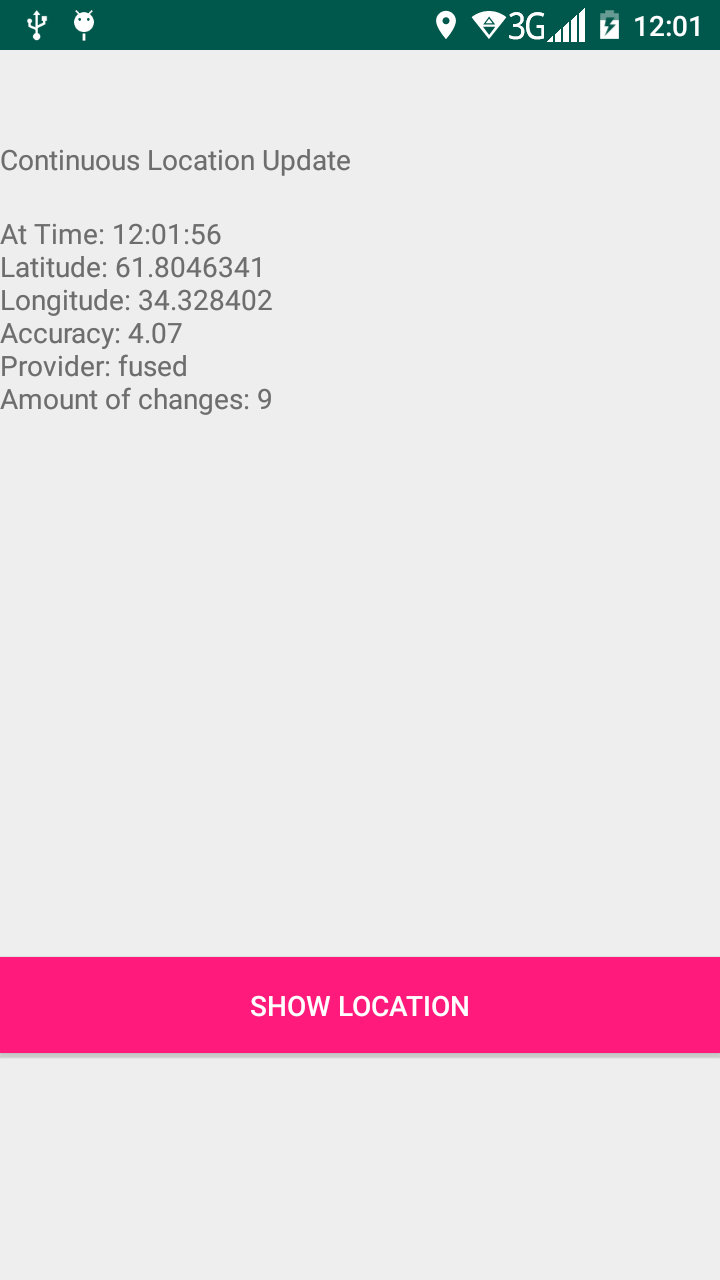
\includegraphics[scale=0.1]{images/Screenshot_2018-12-07-12-01-59.png}
	\end{center}
  
\end{frame}

% Пример заключительного слайда
\begin{frame}
  \frametitle{Заключение}
  
  Полученные результаты
  
  \begin{itemize}
  	\item Изучены базовые принципы разработки мобильных приложений.
  	\item Установлены и настроены инструменты разработки под Android.
  	\item Изучены основные технологии разработки под платформу Android.
  	\item Изучены технологии отслеживания местоположения.
  	\item Написано тестовое приложение без работы в фоне.
  \end{itemize}
  
\end{frame}

\begin{frame}
  \frametitle{}
  
{\Large\mbox{}\hfil Спасибо за внимание!}
  
\end{frame}
\end{document}
